%!TEX root = ../report.tex

\section{Approach}
\label{sec:approach}
In this work, we propose a modular framework for transfer learning in reinforcement learning. 
This framework consists of three modules: 
\begin{enumerate}[i]
    \item the \textbf{representation module}, which constructs an abstract representation of the task environment;
    \item the \textbf{policy learner}, which is a RL learner operating based on the task abstraction created by the representation module;
    \item the \textbf{task environment}, which is the RL task to be solved by the policy learner.
\end{enumerate}
In the following we first present the representation module and the policy module and then depict their interplay in the agent's parallel learning process. The tasks that these different modules are tested on will be introduced in Section \ref{sec:experiments}.

\subsection{Representation Module}
The representation module aims at constructing an abstract and useful generalized representation of the environment's states to facilitate later knowledge transfer. In this work, several architectures are proposed as visualized in Figure \ref{fig:repr_learner} and described in the follwoing subsections. All these architectures follow the pattern of an autoencoder \citep{ballard1987modular} and include some lower-dimensional ``bottleneck'' layers for dimensionality reduction of the input. Autoencoders have shown before to be useful for learning representations \citep{bengio2012deep} in different applications (see e.g. \citet{ap2014autoencoder} and \citet{silberer2014learning} for language or \citet{wang2013learning} for images). We will use the middle layer representation as the latent space projection on which the DDQN learns its policy.
Once learned, this intermediate latent space is expected to create a more compact and abstract representation of the original environment and serve as the basis of transfer learning. This is opposed to previous work that trained the convolutional layers only on the loss produced by the DQN (or, more generally, the policy). We hypothesize the generality of the latent space guided by the representation module to help when transferring knowledge. 

In the following, we will refer to the error calculated based on the heads of the architectures presented below as the \textit{autoencoder loss}. This is to be distinguished from the \textit{policy loss} that is referring to the error calculated by the DDQN.

\begin{figure}[ht!]
	\centering
	\begin{subfigure}{0.45\columnwidth}
		\centering
		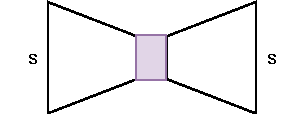
\includegraphics[width=\linewidth]{img/very_simple_autoencoder.pdf}
		\caption{Simple autoencoder}
		\label{subfig:repr_learner_simple_autoencoder}
	\end{subfigure}%
	~ 
	\begin{subfigure}{0.45\columnwidth}
		\centering
		\includegraphics[width=\linewidth]{documentation/report/img/variational_autoencoder_ver2.png}
		\caption{Variational autoencoder}
		\label{subfig:repr_learner_vae}
	\end{subfigure}
	\begin{subfigure}{0.5\columnwidth}
		\centering
		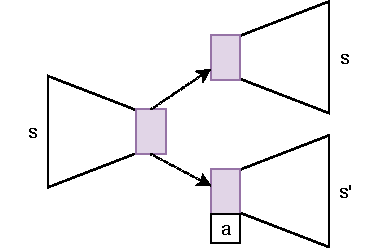
\includegraphics[width=\linewidth]{img/janus.pdf}
		\caption{Janus}
		\label{subfig:repr_learner_janus}
	\end{subfigure}%
	~ 
	\begin{subfigure}{0.5\columnwidth}
		\centering
		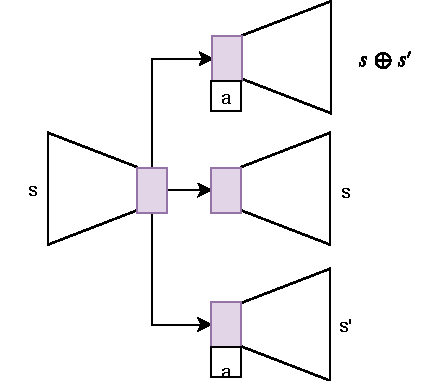
\includegraphics[width=\linewidth]{img/cerberus.pdf}
		\caption{Cerberus}
		\label{subfig:repr_learner_cerberus}
	\end{subfigure}
	\caption{Network architectures of different representation modules, where $s$ and $s'$ indicate current and next state respectively, and $a$ indicates the action leading from $s$ to $s'$. 
	The layers marked in purple are the latent representations to be used as the basis of later transfer learning. 
	The arrows indicate a straight copy from source to target.
	}
	\label{fig:repr_learner}
\end{figure}

\subsubsection{Simple and Variational Autoencoder}
The simplest representation module is the classic autoencoder, which in our case compresses and reconstructs the current state. Figure \ref{subfig:repr_learner_simple_autoencoder} illustrates the \textit{simple autoencoder}.  A modification to this basic model is the so called variational autoencoder (VAE) (see Figure \ref{subfig:repr_learner_vae}). A VAE is a generative approach that models the latent distribution with a Gaussian distribution. Whether it is the simple or variational autoencoder, one theoretical drawback of using such a simple structure for representation learning is that since the latent space only aims at compressing the state and no dynamics of the task are encoded, it is not necessarily a useful basis for learning a policy. The upcoming architectures aim to account for this.

\subsubsection{Janus}
To create more guidance in the construction of the latent space, we add another decoder to capture the dynamics of the environment. As shown in Figure \ref{subfig:repr_learner_janus}, in addition to reconstructing the current state, we also append the action to the representation and seek to use this combination to predict the next state.
The hypothesized effect of this approach is that the latent representation is incentivized to preserve transition dynamics in the environment, and therefore is a more meaningful abstraction of the task.

\subsubsection{Cerberus}
Extending Janus, the Cerberus architecture adds another decoder, which aims at predicting the difference between the current and the next state. By predicting the differences instead of the next state in its entirety, focus is placed on the change caused by the action taken but also the dynamics of the environment in general. We expect this to be especially useful when the changes between consecutive states are small relative to the entire state representation. Optimally, this makes it easier for the encoder to focus on dynamic properties of the environment, such as the position of the agent. The network architecture is shown in Figure \ref{subfig:repr_learner_cerberus}.\\

While it is possible to use both Janus and Cerberus as variational autoencoders, experiments with the simple VAE showed that its representation is most likely too imprecise given the noisy nature of its latent space.

\subsection{Policy Learner}
Based on the latent space constructed by the representation module, the policy learner trains an RL agent to complete a given task. 
%One of the drawbacks of table-based Q-learning occurs in environments with large state spaces. Maintaining and updating the values of all possible states is memory intensive and requires a great amount of training data. An alternative that avoids this problem is function approximation, where Deep-Q-Networks are a popular algorithm.
We use the Double Deep Q-Network \citep{DDQN} algorithm, which is a Q-learning algorithm that uses deep neural networks to approximate the state Q-values of each action.

With the goal of improving and accelerating the learning process, experience replay \citep{replay_memory_oc} is used in conjunction with the algorithm. This mechanism stores the situations that the agent previously encountered as ``memories'' and randomly samples them to train the network. The sampling of memories is meant to remove correlation between training instances and avoid forgetting previous experiences, facilitating learning.

\subsection{Parallel Learning Process}
During training, the agent learns the construction of the latent space and the policy based on the latter in a parallel approach. In each step of every training episode, first the representation module is trained on a batch of observations. Subsequently, the DDQN is updated based on a state-action-reward-state tuple in which the states were encoded into the latent space using the new version of the representation module. 

\paragraph{Batch Representation Learning} To improve the efficiency of training the representation module, batch learning is used. All observations are stored in memory and are fed into the representation network in minibatches of size 32, randomly sampled from this memory. The memory is limited in its size to 1024 observations and dequeues in a \textit{first-in-first-out} manner.

\paragraph{Full backpropagation} Furthermore, when updating the policy, the loss of the DDQN is also backpropagated through the encoder of the representation module. This additionally biases the representation to be sensible to the collected rewards.\\

A parallel approach to learning the two submodules of the agent implicates that during early episodes, the latent states seen by the DDQN are of very low quality. To counteract this, the training involves a warm up period in which the DDQN learns only on single samples without storing them in a memory. Only after a chosen amount of steps the replay memory is going to be filled, assuming that the quality of the memories is now sufficient.

\paragraph{Multi-Task Learning} In multi-task learning, the training alters between the tasks by randomly choosing the next environment at the beginning of each episode. If the observations are given to the DDQN in the same order, this could lead to the agent constantly trying to perform well in the new task, instead of finding a general policy. As a solution we propose an experience stack in which each experience (that is, a state-action-reward-state tuple and the done-flag) is stored when observed. After a warm up period that fills the stack, at each step a random element is popped from the stack and fed to the policy.

\paragraph{Intergradient Learning Phases} In the beginning of training, efficient learning of a useful representation is crucial. In later stages, the representation should only be fine-tuned, since the policy needs to see consistent input. Additionally, the training based on the auto-encoder's loss is supposed to guide the encoder towards representing a generalizable latent space. But when progressing, this guidance should slowly diminish to allow the DDQN to fine-tune the encoder to task-oriented needs. We guarantee such an intergradient learning by introducing a learning rate schedule to the representation module that reduces the learning rate of the auto-encoder by 10 percent every 500 episodes. At the same time the learning rate of the DDQN is kept constant. To speed up learning, we heuristically set 500,000 episodes to be the point at which the learning rate is so small that we can turn off updating based on the autoencoder loss. 

\begin{figure*}[t]
	\centering
	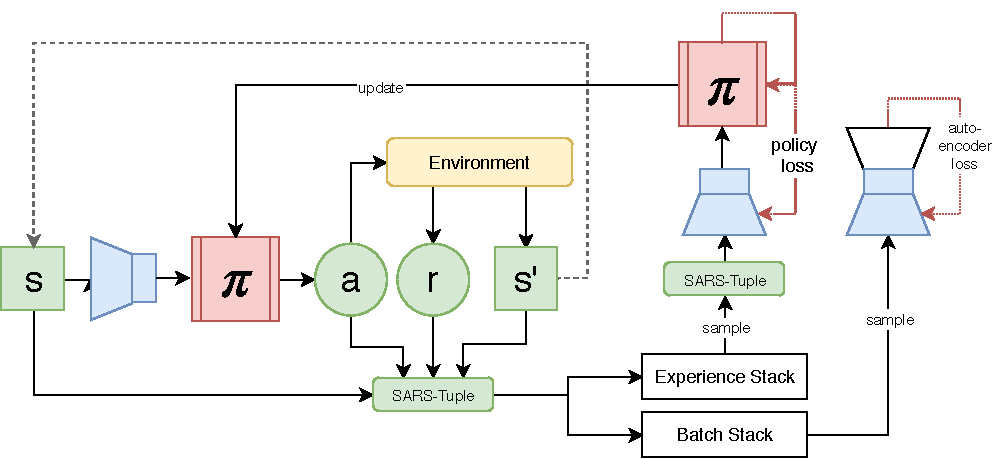
\includegraphics[width=\textwidth]{img/full-model.pdf}
	\caption{Illustration of the parallel approach, where the representation module and policy are trained simultaneously as the agent operates in the environment. At every time step, the current state is given to the current version of the representation module's \textit{encoder} (blue). The resulting latent space representation is used by the current policy (red) to decide on the best action. After executing this action, the environment gives back an immediate reward and the next state. The four-tuple of current state \textit{s}, action \textit{a}, reward \textit{r} and next state \textit{s'} (green) is stored in both an experience stack and a batch stack. From the experience stack, one random tuple is sampled and fed into representation module and subsequently the policy, where a policy loss is calculated and backpropagated through both the DDQN (policy) and the representation module's encoder. This updates the policy used in the next iteration. Furthermore, a batch of 32 tuples is sampled from the batch stack and fed through the full representation module to calculate an autoencoder loss that is backpropagated through the full representation module. Finally, the next state is taken as the current state and the procedure repeats itself. \label{fig:approaches}}
\end{figure*}

% \subsubsection{History Approach}
% As the name indicates, the history approach first creates a collection of states, actions and rewards by randomly exploring in the environment.
% The representation module is then trained based on the collected history.
% Once learning completes, the policy learner is trained based on the encoding of the representation module.
% In this approach, the representation and policy learning are sequential and decoupled. 